% run the command ' lualatex -shell-escape Reference.tex ' twice in the terminal to visualize table of contents
\documentclass[twoside]{article}
% \documentclass{book}
\usepackage[utf8]{inputenc}
\usepackage[english]{babel}
\usepackage{geometry}
\usepackage{multicol}
\usepackage{minted}
\usepackage{python}
\usepackage[hidelinks]{hyperref}
\usepackage{fancyhdr}
\usepackage{listings}
\usepackage{pdfpages}
\usepackage{needspace}
\usepackage{sectsty}
\usepackage{array}
\usepackage{multirow}
\usepackage{longtable}
\usepackage{xcolor}
\usepackage{afterpage}
\usepackage{amssymb}
\usepackage{amsmath}
\usepackage{float}
\usepackage[inline]{enumitem}
\usepackage{fontspec}

\geometry{letterpaper, portrait, left=1cm, right=1cm, top=1.8cm, bottom=1cm}

\setminted{
    style=tango,
		breaklines=true,
		linenos=true
}

\setlength{\headsep}{0.5cm}
\setlength{\columnsep}{0.5cm}
\setlength{\columnseprule}{0.01cm}
\renewcommand{\columnseprulecolor}{\color{gray}}

\pagestyle{fancy}
\pagenumbering{arabic}
\fancyhead{}
\fancyfoot{}
\fancyhead[LO,RE]{\textsf{First, solve the problem. Then, write the code.}}
\fancyhead[LE,RO]{\textsf{\leftmark}}
\fancyfoot[LE,RO]{\textbf{\textsf{\thepage}}}

\renewcommand{\headrulewidth}{0.01cm}
\renewcommand{\footrulewidth}{0.01cm}

\setlength{\parindent}{0em}
% column space
\setlength{\tabcolsep}{10pt} % Default value: 6pt
% upper and lower padding
\renewcommand{\arraystretch}{1.5} % Default value: 1

\definecolor{prussianblue}{rgb}{0.0, 0.19, 0.33}
\definecolor{indigo(dye)}{rgb}{0.0, 0.25, 0.42}
\definecolor{lapislazuli}{rgb}{0.15, 0.38, 0.61}
\definecolor{mediumelectricblue}{rgb}{0.01, 0.31, 0.59}
\definecolor{smalt(darkpowderblue)}{rgb}{0.0, 0.2, 0.6}
\definecolor{yaleblue}{rgb}{0.06, 0.3, 0.57}
\definecolor{skobeloff}{rgb}{0.0, 0.48, 0.45}
\definecolor{pinegreen}{rgb}{0.0, 0.47, 0.44}
\definecolor{lightgray}{gray}{0.9}

\newcommand{\fileTitleStyle}{\centering\underline}

\sectionfont{\centering\bfseries\Huge}
\subsectionfont{\bfseries\LARGE}
\subsubsectionfont{\bfseries\Large}
\paragraphfont{\bfseries\large}

\setmainfont{Montserrat}

\begin{document}
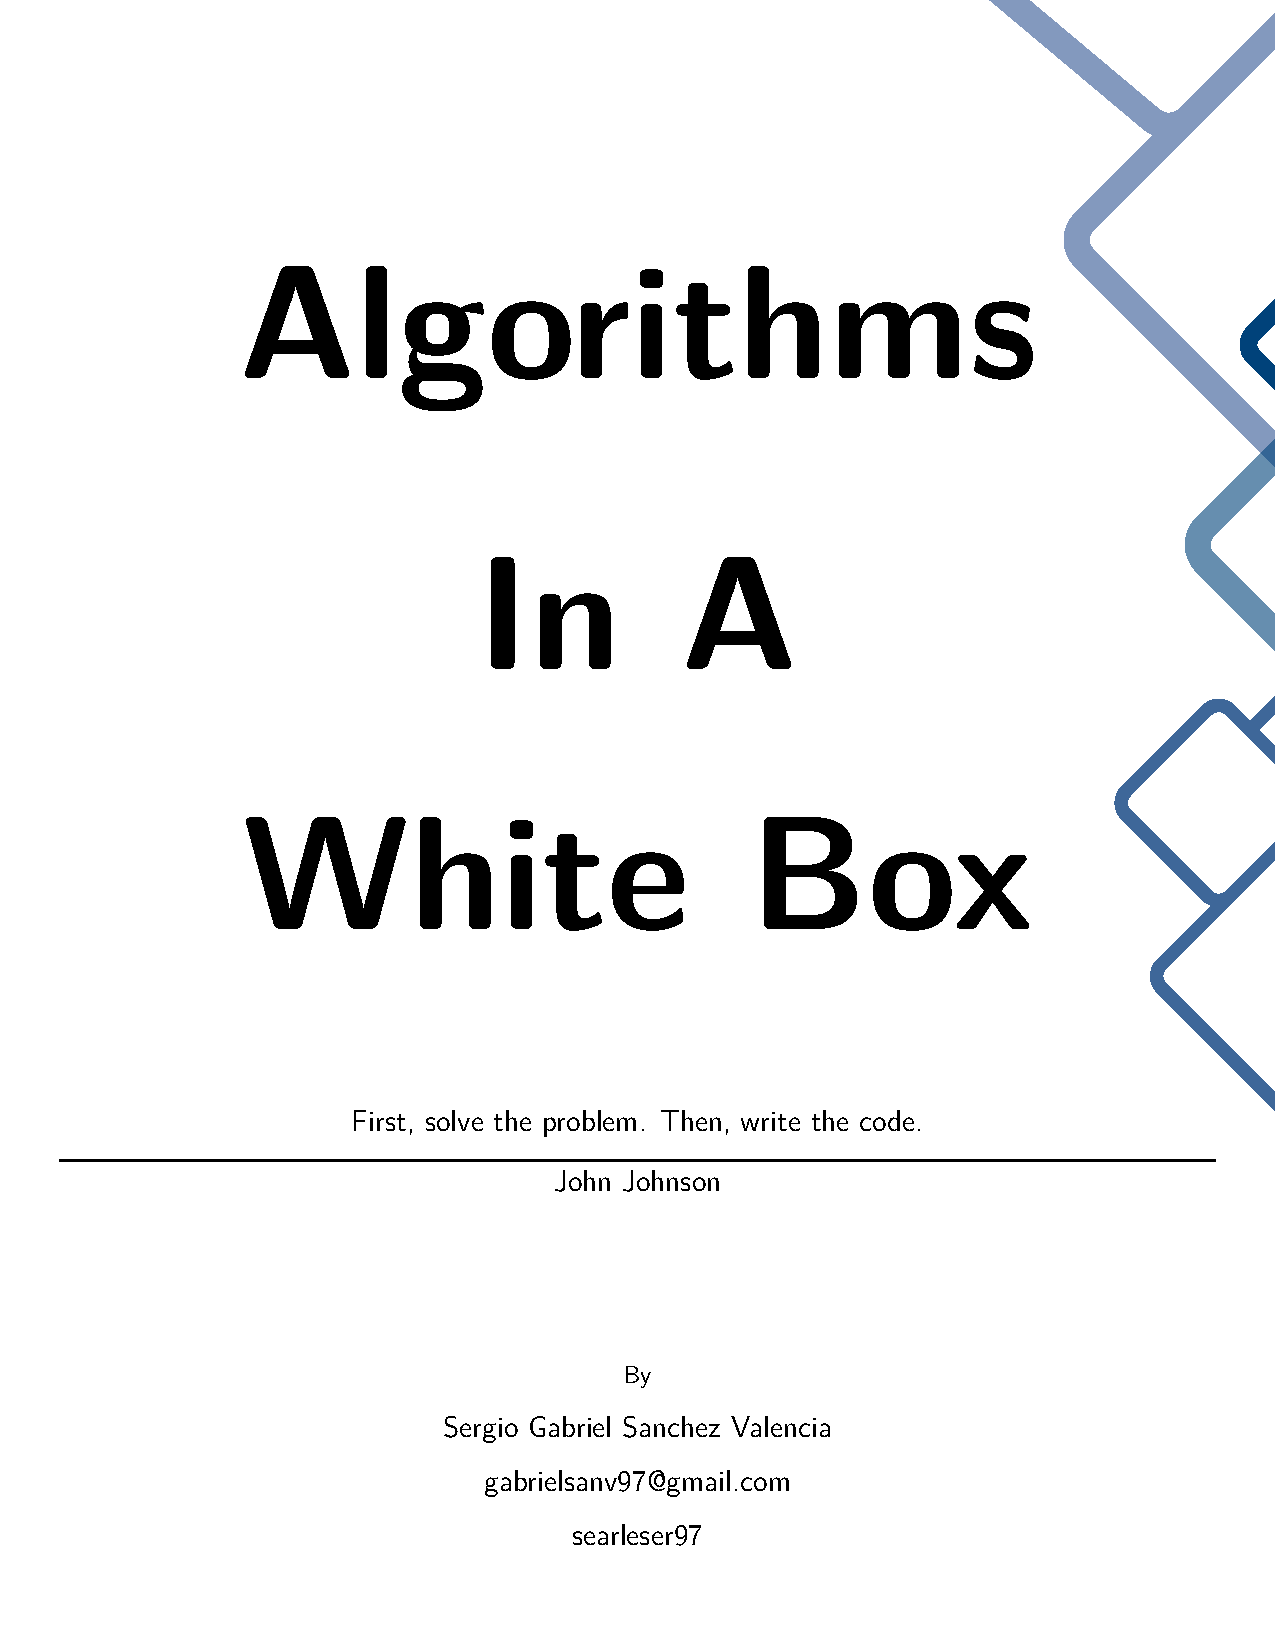
\includepdf{"/home/san/Projects/Algorithms-In-A-White-Box/LaTex Template/TitlePage/TitlePage.pdf"}
\thispagestyle{empty}
\cleardoublepage
\tableofcontents
\newpage
\thispagestyle{empty}
\cleardoublepage
\begin{multicols*}{2}
\end{multicols*}
\newpage
\sectionfont{\centering\bfseries\Huge}
\vspace{1em}
\section*{BITs Manipulation}
\markboth{BITS MANIPULATION}{}
\addcontentsline{toc}{section}{BITs Manipulation}
\vspace{3em}
\subsectionfont{\bfseries\LARGE}
\subsectionfont{\fileTitleStyle}
\subsection*{Least Significant Set Bit}
\addcontentsline{toc}{subsection}{Least Significant Set Bit}
\vspace{1em}
\sffamily
\bgroup

First thing we need to notice is that when we add 1 to a number $N$, what we are doing is just converting the first (right to left) 0-bit into a 1-bit and
the 1-bits before get converted to 0-bits because $1 + 1 = 0$ with carry of $1$ in binary, therefore we will be having a carry of 1-bit until we find a 0-bit.\\

\textbf{Example:}

$$00100111 + 1 = 00101000$$

Second thing we need to notice is very simple, lets start by denoting $\overline{N}$ as $N$ with all it's bits inverted (1-bits change to 0-bit and viceversa), if we perform an $AND$ operation between $N$ and $\overline{N}$ we will get all bits in $0$ as result.\\

\textbf{Example:}

$$N = 00100111$$
$$\overline{N} = 11011000$$

So, to achieve our main objective which is to extract the least significant bit (rightmost bit) we can just invert $N$ and add 1 to it that will convert the first 0-bit to 1-bit so if we make an $AND$ operation with $N$ and $\overline{N}$ we get everything before the lsb as 0-bit and after the lsb we also get everything as 0-bit.\\

And we can write this as the 2's complement since what we did was just to invert bits and add one, which is just the exact definition of 2's complement.\\

\textbf{C++ Code:}\\
\begin{minted}[bgcolor=lightgray]{cpp}
int lsb(int n) {
  return n & -n;
}
\end{minted}

% \begin{figure}[thp]
%   \centering
%   \begin{minipage}[c]{0.2\textwidth}
%     \begin{minted}[bgcolor=lightgray]{cpp}
% int lsb(int n) {
%   return n & -n;
% }
%       \end{minted}
%   \end{minipage}
% \end{figure}

\egroup
\vspace{1em}
\begin{multicols*}{2}
\end{multicols*}
\newpage
\sectionfont{\centering\bfseries\Huge}
\vspace{1em}
\section*{Graph Theory}
\markboth{GRAPH THEORY}{}
\addcontentsline{toc}{section}{Graph Theory}
\vspace{3em}
\subsectionfont{\bfseries\LARGE}
\subsectionfont{\fileTitleStyle}
\subsection*{Articulation Points And Bridges}
\addcontentsline{toc}{subsection}{Articulation Points And Bridges}
\vspace*{2em}
Let's define what an \textit{articulation point} is. We say that a vertex $V$ in a graph $G$ with $C$
connected components is an \textit{articulation point} if its removal increases the number of connected components of $G$.
In other words, let $C'$ be the number of connected components after removing vertex $V$, if $C' > C$ then $V$ is an \textit{articulation point}.

\begin{figure}[H]
  \centering
  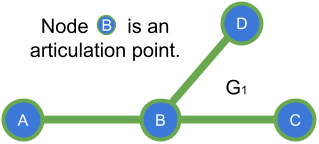
\includegraphics[width=0.3\textwidth]{"Images/Graph Theory/Articulation Points And Bridges/1.png"}
\end{figure}

\subsubsection*{How to find articulation points?}
\bullet Naive approach $O(V * (V + E))$

\begin{minted}{ruby}
for every vertex V in the graph G do
    Remove V from G
    if the number of connected components increases then V is an articulation point
    Add V back to G
\end{minted}
\begin{multicols*}{2}
\end{multicols*}

\end{document}
